\chapter[Second Friend: Conditionals]{Conditionals}

The next thing that you can do is make decisions between alternatives. Conditional logic in your programs simulates decision-making. The common way to decide what to do in JavaScript is to use an if-statement. If-statements will be your second friend! Along the way, we'll meet new data types, including one that allows us to group multiple variables together.

\section{Truthiness}
When deciding between two options---should we go to the beach or stay inside?---we use some criterion to push us to one side or the other---It's hot out, let's go to the beach. We can phrase the process in terms of asking a question and responding with a context-appropriate answer:

Is it hot out?
Yes, let's go to the beach.
No, let's stay inside.

In JavaScript we use the \textsf{Boolean} data type to simulate the answers yes and no. Because \textsf{Boolean} is a data type it has two parts: a collection of values, and a collection of operators that operate on those values. Unlike \textsf{Number} values, there aren't that many distinct \textsf{Boolean} values. In fact, there are only two. They are the literal values \texttt{true} and \texttt{false}. Don't let the fact that there are only two of them fool you. They are immensely powerful and can be combined in very complicated and useful ways. Let's see how.

\begin{question}
  Find and fix the bug in the following line of code.
  \begin{lstlisting}
    let true;
  \end{lstlisting}
\end{question}

There are three built-in operators that transform \textsf{Boolean} values into other \textsf{Boolean} values. They are named logical \textsf{not}, logical \textsf{and}, and logical \textsf{or}. They let you model answers to compound questions. It's easy to get caught up in logic puzzles and every single programmer gets it backwards at some point. But at their core, \textsf{Boolean} expressions involving the so-called logical operators are just answers to questions. And you know how to answer questions. Don't let the foreign programming language syntax make you forget that.

Let's start with the simplest transformer logical \textsf{not}. In JavaScript, the explaination point (\texttt{!})---sometimes pronounced ``bang!'' in programming circles---is used to notate logical \textsf{not} in code. It takes one \textsf{Boolean} input and transforms it into one \textsf{Boolean} output. To describe logical \textsf{not} fully, we can draw its fundamental diagram all of its inputs, i.e., twice: once with the input \texttt{true}, and again with the input \texttt{false}.

\begin{figure}
  \begin{tikzpicture}[node distance=0.75cm, color=cyan, font=\sffamily\small, thick]

  \node[draw, thick, fill=cyan!20, minimum size=2em, inner sep=1em] (transformer) {not};
  \node (inputs) [left of=transformer] {\texttt{true}};
  \node (outputs) [right of=transformer] {\texttt{false}};
  \node (expression) [below=1em of transformer] {\texttt{!true}};

  \draw[->, thick, shorten >= 1em, shorten <= 0.25em] (inputs) -- (transformer);
  \draw[->, thick, shorten >= 0.25em, shorten <= 0.5em] (transformer) -- (outputs);

\end{tikzpicture}
\\
  \begin{scaletikzpicturetowidth}{\textwidth}
  \begin{tikzpicture}[scale=\tikzscale, node distance=3cm, color=cyan, font=\sffamily\small]

    \node[draw, thick, fill=cyan!20, minimum size=2em, inner sep=1em] (transformer) {not};
    \node (inputs) [left of=transformer] {\texttt{false}};
    \node (outputs) [right of=transformer] {\texttt{true}};
    \node (expression) [below=1em of transformer] {\texttt{!false}};

    \draw[->, thick, shorten >= 1em, shorten <= 0.25em] (inputs) -- (transformer);
    \draw[->, thick, shorten >= 0.25em, shorten <= 0.5em] (transformer) -- (outputs);

  \end{tikzpicture}
\end{scaletikzpicturetowidth}

  \caption{\label{conds:not-fundamental-diagram.tex}The fundamental diagrams for logical \textsf{not} applied to each input.}
\end{figure}

Now you (technically) know everything there is to know about the function logical \textsf{not}. When the input is \texttt{true}, the output \textsf{not} \texttt{true} evaluates to the value \texttt{false}. Likewise, when the input is \texttt{false}, the output \textsf{not} \texttt{false} evaluates to \texttt{true}. Logical \textsf{not} flips Boolean values between \texttt{true} and \texttt{false}.

It is somewhat cumbersome to write out the fundamental diagram for each input value to a function. For functions that operate on a small number of inputs, such as these \textsf{Boolean} operators, it is convenient to collect the inputs and outputs into a table, with one column for each input and another column for an expression of function applied to the inputs, and a final column for the evaluation of the expression.

\begin{figure}[h]
  \ttfamily
  \small
  \color{cyan}
  \begin{tabular}{c  c  c}
    x & !x & !x\\
    \textsf{Input} & \textsf{Application} & \textsf{Evaluation}\\
    \hline
    true & !true & false\\
    false & !false & true
  \end{tabular}
  \caption{\label{fig:conditionals-logical-not} The truth table for the function logical \textsf{not}.}
\end{figure}

You can create such a table for any function. But when you create this kind of table for combinations of \textsf{Boolean} functions, it gets a special name: a \emph{truth table}. It is extremely easy to get confused when working through the value of a \textsf{Boolean} expression. Even very experienced programmers will get tripped out.\marginnote{Always write things down. Don't try to calculate in your head. You don't get bonus points for doing it in your head.} Truth tables are extremely helpful at making the logic of an expression plain, especially once we start combining operators to make more complicated expressions.

\begin{question}
  Write the pipeline fundamental diagram of the function double \textsf{not} (\texttt{!!}); that is, the function of \textsf{not} applied to the output of \textsf{not}.
\end{question}

\begin{question}
  Write the truth table for double \textsf{not} (\texttt{!!}). \textsc{Hint:} For any input \texttt{x}, \texttt{!!x} evaluate to the same value as \texttt{!(!x)}; that is, the value of \textsf{not} applied to the output of \textsf{not}.
\end{question}

When calculating the value of a boolean expression is very, very helpful to break it down into as many subexpressions as possible. As an example, let's construct the truth table for triple \textsf{not} (\texttt{!!!}). We'd like to be able to write down the answer straight away, but that involves a lot of intermediate calculations. If we tried to keep track of things in our head, it'd be easy to lose track of how many times we've applied \textsf{not}. So, let's expand our table to include all of the intermediate calculations. \marginnote{When working on pipelines with big data, saving intermediate steps becomes even more critical. If the pipeline fails after running for days on a large data set, you'll be happy that you saved intermediate steps instead of starting over at the beginning. Your boss will be happy that you did, too.} It is good and be explicit and write down all of the steps.

Let's make a dummy variable \texttt{x} to be in the input of our expression. In one row, \texttt{x} will be assigned the value \texttt{true}. In the other, \texttt{x} will be assigned the value \texttt{false}. We want to know what the output value \texttt{!!!x} evaluates to. In order to calculate \texttt{!!!x}, we first need to calculate \texttt{!!x}. But to calculate \texttt{!!x}, we first need to calculate \texttt{!x}. But we know how to calculate \texttt{!x}. Let's go!

\begin{figure*}[h]
  \ttfamily
  \color{cyan}
  \small
  \begin{tabular}{c c c c c c c}
    x & !x & !x & !(!x) & !(!x) & !(!!x) & !(!!x) \\
    \textsf{Input} & \textsf{Application} & \textsf{Evaluation} & \textsf{Application} & \textsf{Evaluation} & \textsf{Application} & \textsf{Evaluation}\\
    \hline
    true & !true & false & !false & true & !true & false\\
    false & !false & true & !true & false & !false & true
  \end{tabular}
  \caption{\label{fig:conditional-triple-not-table}The truth table for triple \textsf{not}, with intermediate calculations for subexpressions.}
\end{figure*}

Logical \textsf{not} produces a single \textsf{Boolean} output. When we repeatedly apply \textsf{not}, we can temporarily forget about that all of the other \textsf{not}s to come and focus on the inputs and outputs one at a time. In general, to evaluate an expression (of any kind), we evaluate the nearest function on its input and work to the outside, providing the output of one function as the input to the next. While we could draw a fundamental diagram each time we supply outputs as inputs, we often use parentheses to signify the inputs. Below we've written out the top row of the truth table for triple-\textsf{not} with parentheses to point out which step we're working on. After each applicaion of \textsf{not}, the expression reduces to a simpler one. Then we pass on the output to the next copy of \textsf{not} for evaluation. Each time, moving the parentheses over by one place to capture the next function application. This process of grouping inputs and moving to the next function will work for all expressions, not just \textsf{Boolean} expressions. And we will use this technique widely for the rest of programming for all time.

\begin{figure*}[h]
  \ttfamily
  \color{cyan}
  \small
  \begin{center}
  !!!true $\to$ !!(!true) $\to$ !!(false) $\to$ !(!false) $\to$ !(true) $\to$ (!true) $\to$  false
  \end{center}
  \caption{This is a margin figure.}
\end{figure*}

Logical \textsf{not} takes only on input. The other two \textsf{Boolean} functions, logical \textsf{or} and logical \textsf{and}, operate on two inputs.

\begin{marginfigure}
  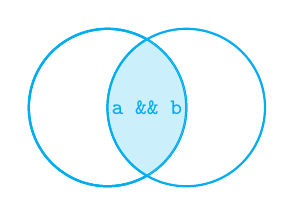
\begin{tikzpicture}[node distance=0.75cm, color=cyan, font=\ttfamily\footnotesize, thick]

  \draw (0, 0) circle (1);
  % \draw (-0.5, 0) node {a};

  \draw (1, 0) circle (1);
  % \draw (1.5, 0) node {b};

  \begin{scope}
    \draw[clip] (0,0) circle (1);
    \fill[cyan!20] (1,0) circle (1);

    \draw (0,0) circle (1);
    \draw (1,0) circle (1);
  \end{scope}

  \draw (0.5, 0) node {a \&\& b};

\end{tikzpicture}

  \caption{Logical \textsf{and} is \texttt{true} only when both \texttt{a} is \texttt{true} and \texttt{b} is \texttt{true}. You can visualize it as the instances where \texttt{a} and \texttt{b} coincide.}
\end{marginfigure}

\begin{marginfigure}
  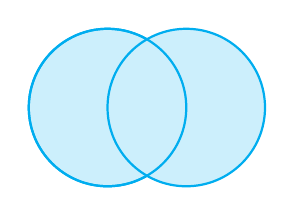
\begin{tikzpicture}[node distance=0.75cm, color=cyan, font=\sffamily\small, thick]

  \filldraw[fill=cyan!20] (0, 0) circle (1cm);
  \filldraw[fill=cyan!20] (1, 0) circle (1cm);
  \draw (0,0) circle (1cm);

\end{tikzpicture}

  \caption{Logical \textsf{or} is \texttt{true} when either \texttt{a} is \texttt{true} or \texttt{b} is \texttt{true}. You can visualize it as all the instances of \texttt{a} and \texttt{b} combined.}
\end{marginfigure}

\begin{marginfigure}
  
\begin{tikzpicture}[node distance=0.75cm, color=cyan, font=\ttfamily\small, thick]

  \fill[cyan!20] (-2, -1.25) rectangle (2, 1.25);
  \filldraw[fill=white, thick] (0, 0) circle (1);
  \draw (1.5, -0.8) node {!a};

\end{tikzpicture}

  \caption{Logical \textsf{not} is \texttt{true} whenever \texttt{a} is \texttt{false}. You can visualize it as all the instances that are not instances of \texttt{a}.}
\end{marginfigure}

\begin{itemize}
  \item boolean data types
  \item comparison operators
  \item transformers can convert one type to another type. that's the transform part! (transformers are stateless?)
  \item equality operators
  \item if statements
  \item scope
  \item running programs
  \item using libraries
  \item command-line arguments
  \item arrays --- multiple values
  \item difference between identity and equality (memory and reference types)
  \item arrays as look-up tables
  \item arrays conditional execution
  \item arrays as finite functions
\end{itemize}
